\documentclass[12pt]{article}

% Packages for math and formatting
\usepackage[utf8]{inputenc}
\usepackage{amsmath, amssymb, amsthm}   % math symbols & environments
\usepackage{geometry}                   % page layout
\usepackage{enumitem}                   % better lists
\usepackage{hyperref}                   % clickable references
\usepackage{mathtools}                  % extended math tools
\usepackage{epigraph}                   % for quotes
\usepackage{tikz}
\usetikzlibrary{arrows.meta}


% Page setup
\geometry{margin=1in}

% Theorem-like environments
\newtheorem{theorem}{Theorem}[section]
\newtheorem{proposition}[theorem]{Proposition}
\newtheorem{lemma}[theorem]{Lemma}
\newtheorem{corollary}[theorem]{Corollary}
\theoremstyle{definition}
\newtheorem{definition}[theorem]{Definition}
\newtheorem{problem}[theorem]{Problem}
\theoremstyle{remark}
\newtheorem{remark}[theorem]{Remark}
\newtheorem{example}[theorem]{Example}

% Custom commands
\newcommand{\R}{\mathbb{R}}
\newcommand{\N}{\mathbb{N}}
\newcommand{\Q}{\mathbb{Q}}
\newcommand{\Z}{\mathbb{Z}}
\newcommand{\C}{\mathbb{C}}
\newcommand{\PP}{\mathbb{P}}
\newcommand{\D}{\mathbb{D}}
% Linear groups
\newcommand{\GL}{\operatorname{GL}}

\newcommand{\HH}{\mathbb{H}} % upper half-plane

\DeclareMathOperator{\Aut}{Aut}
\DeclareMathOperator{\FractLin}{FractLin}
\DeclareMathOperator{\ord}{ord}
\DeclareMathOperator{\Res}{Res}
\DeclareMathOperator{\SL}{SL}

\title{Elliptic Functions, Part 1}
\author{Joe}
\date{September 17, 2025}

\begin{document}
	
	\maketitle
	
	\tableofcontents
\vspace{1em}
	
	\section{Compact Riemann Surfaces of Genus 1 and Lattices}
	
	\begin{definition}[Genus]
		The genus $g(X)$ of a compact Riemann surface $X$ is a topological invariant that counts the number of ``holes'' in the surface. 
		\begin{itemize}
			\item $g=0$: the Riemann sphere $\PP^1$ (no holes),
			\item $g=1$: a torus (one hole),
			\item in general, $g$ holes correspond to a $g$‑torus.
		\end{itemize}
		Thus, a genus $1$ compact Riemann surface is topologically a torus.
	\end{definition}
	
	\begin{definition}[Universal Cover]
		Let $X$ be a connected topological space. A \emph{universal cover} of $X$ is a simply connected space 
		\[
		\pi : \tilde{X} \to X
		\]
		such that every covering of $X$ factors through $\pi$. Here ``simply connected'' means $\pi_1(\tilde{X}) = 0$, i.e.\ $\tilde{X}$ has no nontrivial loops.
	\end{definition}
	
	\begin{example}
		The universal cover of the circle $S^1$ is $\R$ with covering map $\pi(t) = e^{2\pi i t}$.  
		
		The universal cover of a torus is $\R^2$, with covering map given by projection $\R^2 \to \R^2 / \Z^2$.
	\end{example}
	
	\begin{theorem}[Uniformization Theorem]
		Let $X$ be a simply connected Riemann surface. Then $X$ is biholomorphically equivalent to exactly one of:
		\begin{enumerate}
			\item $\PP^1$ (the Riemann sphere),
			\item $\C$ (the complex plane),
			\item $\D = \{z \in \C : |z| < 1\}$ (the unit disk).
		\end{enumerate}
	\end{theorem}
	
	\begin{proposition}
		If $X$ is a compact Riemann surface of genus $1$, then its universal cover is $\C$.
	\end{proposition}
	
	\begin{proof}
		By the Uniformization Theorem, the universal cover $\tilde{X}$ of $X$ is biholomorphic to one of $\PP^1$, $\C$, or $\D$.  
		
		Suppose first that $\tilde{X} = \PP^1$. Then $X$ would arise as a quotient of $\PP^1$ by a discrete group of automorphisms. Since $\PP^1$ is simply connected of genus $0$, no such quotient can produce a compact Riemann surface of genus $1$.  
		
		Next, suppose $\tilde{X} = \D$. Quotients of the unit disk by discrete groups of automorphisms carry a hyperbolic metric and yield compact Riemann surfaces of genus at least $2$. Hence this case is also impossible for $X$.  
		
		The only remaining possibility is that $\tilde{X} \cong \C$, and therefore the universal cover of a genus $1$ compact Riemann surface is biholomorphic to $\C$.
	\end{proof}
	
	\begin{definition}[Lattice]
		A \emph{lattice} in $\C$ is a discrete additive subgroup of the form
		\[
		L = \Z \omega_1 + \Z \omega_2 = 
		\{ m\omega_1 + n\omega_2 : m,n \in \Z \},
		\]
		where $\omega_1,\omega_2 \in \C$ are linearly independent over $\R$.
	\end{definition}
	
	\begin{proposition}
		Let $\Gamma \subset \Aut(\C)$ be a discrete subgroup acting freely on $\C$. Then exactly two cases can occur:
		\begin{enumerate}
			\item $\Gamma$ is generated by one element. In this case, $\Gamma = \{ n\omega : n\in\Z \}$ for some $\omega \neq 0$, and the quotient $\C/\Gamma$ is biholomorphic to $\C^{\times}$, which is not compact.  
			\item $\Gamma$ is generated by two $\R$--linearly independent elements $\omega_1, \omega_2 \in \C$. In this case
			\[
			\Gamma = L = \Z \omega_1 + \Z \omega_2 ,
			\]
			which is a lattice in $\C$, and the quotient $\C/L$ is a compact Riemann surface of genus $1$.
		\end{enumerate}
	\end{proposition}
	
	\begin{proof}
		We first note that 
		\[
		\Aut(\C) = \{ \phi(z) = az + b : a \in \C^{\times},\; b \in \C \}.
		\]
		If $a \neq 1$, then $\phi(z) = az+b$ has a fixed point $z_0 = b/(1-a)$. Since $\Gamma$ must act freely, such maps cannot occur in $\Gamma$. Therefore every nontrivial element of $\Gamma$ must be a translation of the form $z \mapsto z + \ell$.  
		
		If $\Gamma$ is generated by a single nonzero element $\omega$, then the exponential map 
		\[
		\exp : \C \to \C^{\times}, \qquad z \mapsto e^z
		\]
		has kernel $2\pi i \Z$, showing that $\C/\Gamma \cong \C^{\times}$. This surface is non‑compact and has genus $0$.  
		
		If $\Gamma$ has two $\R$--linearly independent generators $\omega_1, \omega_2$, then $\Gamma$ is a lattice $L = \Z\omega_1 + \Z\omega_2$. The quotient $\C/L$ is compact, since the fundamental parallelogram 
		\[
		\{ a\omega_1 + b\omega_2 : 0 \leq a,b < 1 \}
		\]
		maps bijectively to the quotient space. Topologically this quotient is a torus, hence a compact genus $1$ Riemann surface. No other possibility for $\Gamma$ exists.
	\end{proof}
	
	\begin{corollary}
		Every compact Riemann surface $X$ of genus $1$ is isomorphic to a quotient
		\[
		X \cong \C / L,
		\]
		where $L \subset \C$ is a lattice of rank $2$.
	\end{corollary}
	
	\begin{proof}
		This follows directly from the preceding proposition and the fact that the universal cover of a genus $1$ compact Riemann surface is $\C$.
	\end{proof}
	
	
	
	
	
\begin{theorem}[Moduli of elliptic curves]
	Let $\tau \in \HH := \{ z \in \C : \Im z > 0 \}$ and define the lattice
	\[
	L_\tau = \Z + \Z \tau,
	\]
	together with the elliptic curve (torus)
	\[
	X_\tau := \C / L_\tau.
	\]
	Then two elliptic curves $X_\tau$ and $X_{\tau'}$ are biholomorphic if and only if there exists a matrix
	\[
	\begin{pmatrix} a & b \\ c & d \end{pmatrix} \in \SL(2,\Z)
	\]
	such that
	\[
	\tau' = \frac{a\tau+b}{c\tau+d}.
	\]
	Consequently, the moduli space of compact Riemann surfaces of genus $1$ is
	\[
	\mathcal{M}_1 \;\cong\; \HH / \SL(2,\Z).
	\]
\end{theorem}

\begin{proof}
	Every lattice in $\C$ has the form $L = \Z \omega_1 + \Z \omega_2$ with $\Im(\omega_2/\omega_1) > 0$.  
	Scaling by $\omega_1^{-1}$ yields
	\[
	L = \omega_1 (\Z + \Z \tfrac{\omega_2}{\omega_1}) = \omega_1 L_\tau, 
	\quad\tau = \frac{\omega_2}{\omega_1} \in \HH.
	\]
	Since multiplication by $\omega_1$ gives a biholomorphism $\C/L_\tau \to \C/L$, any elliptic curve is isomorphic to one of the form $X_\tau$.
	
	Suppose $X_\tau \cong X_{\tau'}$. Then there exists a biholomorphism $f: \C/L_\tau \to \C/L_{\tau'}$. Lifting to the universal cover, we get a biholomorphism $\tilde{f}: \C \to \C$ such that $\tilde{f}(L_\tau) = L_{\tau'}$. Since $\Aut(\C)$ consists of affine transformations $z \mapsto az + b$, and $\tilde{f}$ must map lattice to lattice, we have $\tilde{f}(z) = \alpha z$ for some $\alpha \in \C^\times$.
	
	Therefore $L_{\tau'} = \alpha L_\tau$, which means
	\[
	\{\alpha, \alpha\tau\} = \{1, \tau'\}
	\]
	as $\Z$-bases. This gives us two cases:
	\begin{enumerate}
		\item $\alpha = 1$ and $\alpha\tau = \tau'$, so $\tau' = \tau$.
		\item $\alpha = \tau'$ and $\alpha\tau = 1$, so $\tau' \tau = 1$, giving $\tau' = -1/\tau$.
	\end{enumerate}
	
	More generally, there exists a matrix $\begin{pmatrix} a & b \\ c & d \end{pmatrix} \in \GL(2,\Z)$ such that
	\[
	\begin{pmatrix} 1 \\ \tau' \end{pmatrix} = \alpha \begin{pmatrix} a & b \\ c & d \end{pmatrix} \begin{pmatrix} 1 \\ \tau \end{pmatrix} = \alpha \begin{pmatrix} a + b\tau \\ c + d\tau \end{pmatrix}.
	\]
	
	This gives us $1 = \alpha(a + b\tau)$ and $\tau' = \alpha(c + d\tau)$. Solving for $\alpha$ and substituting:
	\[
	\tau' = \frac{c + d\tau}{a + b\tau} = \frac{d\tau + c}{b\tau + a} = \frac{a\tau + c}{b\tau + d}
	\]
	(after swapping $a \leftrightarrow d$ and $b \leftrightarrow c$).
	
	Since both lattices have the same orientation in $\C$, we need $\det \begin{pmatrix} a & c \\ b & d \end{pmatrix} = ad - bc = 1$, so the matrix is in $\SL(2,\Z)$.
	
	Conversely, if $\tau' = \frac{a\tau+b}{c\tau+d}$ for some $\begin{pmatrix} a & b \\ c & d \end{pmatrix} \in \SL(2,\Z)$, then the map $z \mapsto (c\tau + d)z$ gives an isomorphism between $X_\tau$ and $X_{\tau'}$.
	
	Therefore the set of isomorphism classes of compact genus $1$ Riemann surfaces is exactly $\HH/\SL(2,\Z)$.
\end{proof}




\section{Meromorphic Functions on Elliptic Curves}

\subsection{Elliptic Functions and the Construction Problem}
Now fix a lattice $L = \Z\omega_1 + \Z\omega_2$, where $\omega_1$ and $\omega_2$ are linearly independent over $\R$. Write $X = \C/L$.

\noindent \textbf{Objective:} To study $\mathcal{M}(X)$, the field of meromorphic functions on $X$, and answer three principal questions.

\begin{problem}[Question 1]\label{Q1}
	Find an example of $f \in \mathcal{M}(X)$ with $f \not\equiv 0$.
\end{problem}

\begin{remark}
	Since $X = \C/L$ is compact, any holomorphic function on $X$ must be constant by Liouville's theorem. Therefore, all non-constant meromorphic functions on $X$ must have poles.
\end{remark}

\begin{center}
	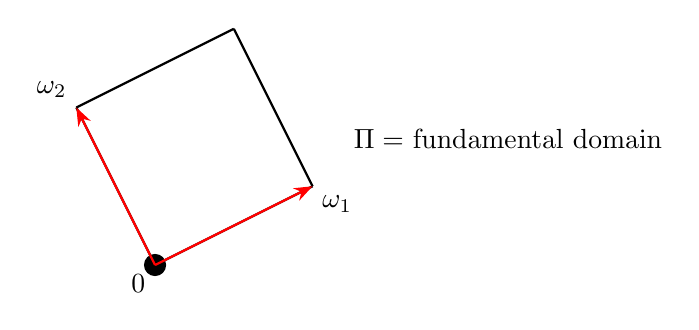
\begin{tikzpicture}[scale=2]
		% Draw the fundamental parallelogram with four lines
		\draw[thick] (0,0) -- (1,0.5);
		\draw[thick] (0,0) -- (-0.5,1);
		\draw[thick] (1,0.5) -- (0.5,1.5);
		\draw[thick] (-0.5,1) -- (0.5,1.5);
		
		% Mark the origin
		\fill[black] (0,0) circle (2pt);
		\node[below left] at (0,0) {$0$};
		
		% Label the lattice vectors
		\draw[-{Stealth}, thick, red] (0,0) -- (1,0.5);
		\node[below right] at (1,0.5) {$\omega_1$};
		
		\draw[-{Stealth}, thick, red] (0,0) -- (-0.5,1);
		\node[above left] at (-0.5,1) {$\omega_2$};
		
		% Add fundamental domain label
		\node[right] at (1.2,0.8) {$\Pi = $ fundamental domain};
	\end{tikzpicture}
\end{center}



\begin{definition}
	An \emph{elliptic function} with respect to a lattice $L \subset \C$ is a meromorphic function
	\[
	f : \C \longrightarrow \C \cup \{\infty\}
	\]
	such that
	\[
	f(z + w) = f(z) \quad \text{for all } z \in \C, \ w \in L.
	\]
\end{definition}



\begin{remark}
	Equivalently, an elliptic function is a \emph{doubly periodic} meromorphic function with respect to $L$.  
	That is, if $L = \Z \omega_1 + \Z \omega_2$ with $\omega_1, \omega_2$ linearly independent over $\R$, then
	\[
	f(z + \omega_1) = f(z), \qquad f(z + \omega_2) = f(z) \quad \text{for all } z \in \C.
	\]
	By linearity this implies
	\[
	f\bigl(z + n_1 \omega_1 + n_2 \omega_2 \bigr) = f(z)
	\quad \text{for all } z \in \C, \ n_1,n_2 \in \Z.
	\]
\end{remark}


\noindent
We denote by $\PP^1 = \C \cup \{\infty\}$ the Riemann sphere, and recall that the elliptic curve associated to a lattice $L$ is the quotient $X = \C / L$.

\medskip

\noindent\textbf{Convention.} 
Strictly speaking, an elliptic function is a meromorphic and doubly periodic function 
\[
f : \C \longrightarrow \PP^1
\]
with respect to $L$.  
However, since $f(z+w) = f(z)$ for all $w \in L$, the function is invariant under translations by elements of $L$.  
Therefore $f$ descends to a well-defined meromorphic function on the quotient $X$: 
\[
f \in \mathcal{M}(X).
\]
In this way, we usually regard elliptic functions as precisely the meromorphic functions on $X$.\\


To answer Problem~\ref{Q1}, we want an explicit example of a nonconstant meromorphic function 
\[
f \in \mathcal{M}(X), \quad f \not\equiv 0.
\]

\medskip

\noindent
A general strategy is the following: if $\Gamma$ is a finite group acting on $\C$ and $h$ is any function on $\C$, then we may form the averaged function
\[
h^*(z) := \sum_{\gamma \in \Gamma} h(\gamma z).
\]

\begin{lemma}
	The function $h^*$ is invariant under the action of $\Gamma$, i.e.
	\[
	h^*(\gamma_0 z) = h^*(z) \qquad \text{for all } \gamma_0 \in \Gamma.
	\]
\end{lemma}

\begin{proof}
	Fix $\gamma_0 \in \Gamma$. Then
	\[
	h^*(\gamma_0 z) 
	= \sum_{\mu \in \Gamma} h\bigl(\mu(\gamma_0 z)\bigr) 
	= \sum_{\mu \in \Gamma} h\bigl((\mu \gamma_0)(z)\bigr).
	\]
	Since $\mu \mapsto \mu \gamma_0$ permutes the group $\Gamma$, this sum can be rewritten
	\[
	\sum_{\nu \in \Gamma} h(\nu z) = h^*(z).
	\]
\end{proof}

\subsection{Eisenstein Series}

\begin{theorem}[Convergence of Lattice Power Sums]\label{thm:lattice-convergence}
	Given an ``appropriate function" $h$ on $\C$, we try to define $f(z) = \sum_{w \in L} h(z+w)$, which is well-defined if $\sum_{w \in L} |h(z+w)| < \infty$.
	
	Take $h(z) = \frac{1}{z^k}$. Then $\sum_{w \in L} \left|\frac{1}{(z+w)^k}\right|$ converges if and only if $k \geq 3$.
	
	\begin{proof}
		Write $w = n_1\omega_1 + n_2\omega_2$ for lattice points. Define:
		\begin{align}
			S_0 &= \{0\} \\
			S_1 &= \{n_1\omega_1 + n_2\omega_2 : -1 \leq n_1, n_2 \leq 1\} \\
			T_1 &= S_1 \setminus S_0 = \{n_1\omega_1 + n_2\omega_2 : n_1 = \pm 1 \text{ or } n_2 = \pm 1\} \\
			S_2 &= \{n_1\omega_1 + n_2\omega_2 : -2 \leq n_1, n_2 \leq 2\} \\
			T_2 &= S_2 \setminus S_1 = \{n_1\omega_1 + n_2\omega_2 : n_1 = \pm 2 \text{ or } n_2 = \pm 2\}
		\end{align}
		More generally, $T_n = S_n \setminus S_{n-1}$ for $n \geq 1$.
		
\begin{figure}[h]
	\centering
	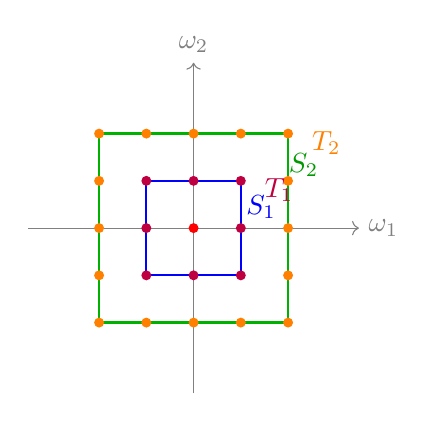
\begin{tikzpicture}[scale=0.6]
		
		% axes
		\draw[->, thin, gray] (-3.5,0)--(3.5,0) node[right]{$\omega_1$};
		\draw[->, thin, gray] (0,-3.5)--(0,3.5) node[above]{$\omega_2$};
		
		% lattice points in S2
		\foreach \i in {-2,...,2}{
			\foreach \j in {-2,...,2}{
				\fill[black] (\i,\j) circle (2pt);
			}
		}
		
		% origin
		\fill[red] (0,0) circle (3pt);
		
		% S1 boundary
		\draw[blue, thick] (-1,-1) rectangle (1,1) node[pos=.95,below right,blue] {$S_1$};
		
		% S2 boundary
		\draw[green!70!black, thick] (-2,-2) rectangle (2,2) node[pos=.95,below right,green!60!black] {$S_2$};
		
		% highlight T2 = S2 \ S1 (outer boundary S2)
		\foreach \i in {-2,...,2}{
			\fill[orange] (\i,-2) circle (3pt);
			\fill[orange] (\i,2) circle (3pt);
		}
		\foreach \j in {-1,...,1}{
			\fill[orange] (-2,\j) circle (3pt);
			\fill[orange] (2,\j) circle (3pt);
		}
		\node[orange,anchor=west] at (2.3,1.8) {$T_2$};
		
		% highlight T1 = S1 \ S0 (boundary of S1)
		\foreach \i in {-1,...,1}{
			\fill[purple] (\i,-1) circle (3pt);
			\fill[purple] (\i,1) circle (3pt);
		}
		\foreach \j in {0}{
			\fill[purple] (-1,\j) circle (3pt);
			\fill[purple] (1,\j) circle (3pt);
		}
		\node[purple,anchor=west] at (1.3,0.8) {$T_1$};
		
	\end{tikzpicture}
	\caption{Lattice points for $S_2$. The red point is the origin. $S_1$ (blue square) and $S_2$ (green square) are shown.
		The purple points form $T_1 = S_1\setminus S_0$, and the orange points form $T_2 = S_2\setminus S_1$.}
\end{figure}
		
		We have $|S_n| = (2n+1)^2$ and $|T_n| = |S_n \setminus S_{n-1}| = 8n$ for $n \geq 1$.
		
		Let $z \notin L$. The question becomes: when is $\sum_{n=0}^{\infty}\sum_{w \in T_n}\left|\frac{1}{(w+z)^k}\right| < \infty$?
		
		Fix $z_0 \notin L$. The question is the same as asking when $\sum_{w \in L^\times}\frac{1}{|w|^k} < \infty$, where $L^\times = L \setminus \{0\}$.
		
		To be more precise, we can write:
		\[
		\sum_{n=0}^{\infty}\sum_{w \in T_n}\left|\frac{1}{(z_0+w)^k}\right| = \sum_{n=0}^{s}\sum_{w \in T_n}\left|\frac{1}{(z_0+w)^k}\right| + \sum_{n=s+1}^{\infty}\sum_{w \in T_n}\left|\frac{1}{(z_0+w)^k}\right|
		\]
		
		For sufficiently large $s$, we have $\forall n \geq s+1, \forall w \in T_n$:
		\[
		\frac{|w|}{2} < |z_0 + w| < \frac{3}{2}|w|
		\]
		by applying the triangle inequality. Then there exist constants $c_1, c_2 > 0$ such that:
		\[
		c_1\sum_{n=s+1}^{\infty}\sum_{w \in T_n}\frac{1}{|w|^k} \leq \sum_{n=s+1}^{\infty}\sum_{w \in T_n}\frac{1}{|z_0+w|^k} \leq c_2\sum_{n=s+1}^{\infty}\sum_{w \in T_n}\frac{1}{|w|^k}
		\]
		
		Hence the absolute convergence of $\sum_{w \in L}\left|\frac{1}{(z_0+w)^k}\right|$ holds if and only if $\sum_{w \in L^\times}\frac{1}{|w|^k} < \infty$.
		
		There exist constants $a, b > 0$ such that $\forall w \in T_n$: $an \leq |w| \leq bn$. To check this for $T_1$, write $\Pi_1$ for the first parallelogram so that $T_1 \subset \partial\Pi_1$ and $T_n \subset \partial\Pi_n$ where $\Pi_n = \{nz : z \in \Pi_1\}$.
		
		If we choose $a, b > 0$ such that:
		\begin{align}
			a &= \min_{\xi \in \partial\Pi_1} |\xi| \\
			b &= \max_{\xi \in \partial\Pi_1} |\xi|
		\end{align}
		then $a \leq \frac{|w|}{n} \leq b$, so $an \leq |w| \leq bn$ holds for all $w \in T_n$, since $T_n \subset \partial\Pi_n$ and $w \in T_n \Rightarrow \frac{w}{n} \in \partial\Pi_1$.
		
		Hence:
		\begin{align}
			\frac{1}{b^k}\left(\sum_{n=1}^{\infty} \frac{8n}{n^k}\right) &\leq \sum_{w \in L^\times} \frac{1}{|w|^k} \leq \frac{1}{a^k}\left(\sum_{n=1}^{\infty}\frac{8n}{n^k}\right) \\
			\frac{8}{b^k}\left(\sum_{n=1}^{\infty} \frac{1}{n^{k-1}}\right) &\leq \sum_{w \in L^\times} \frac{1}{|w|^k} \leq \frac{8}{a^k}\left(\sum_{n=1}^{\infty} \frac{1}{n^{k-1}}\right)
		\end{align}
		
		Conclusion: $\sum_{w \in L^\times}\frac{1}{|w|^k} < \infty \Leftrightarrow k-1 \geq 2$, i.e., $k \geq 3$.
	\end{proof}
\end{theorem}

\begin{corollary}[Eisenstein Series Construction]\label{cor:eisenstein}
	When $k \geq 3$, we can define the \emph{Eisenstein series}:
	\[
	E_k(z) = \sum_{w \in L} \frac{1}{(z+w)^k}
	\]
	where $E$ stands for Eisenstein.
	
\noindent The function $E_k$ has a pole of order $k$ at lattice points and no other poles. Moreover, $E_k$ is doubly periodic with respect to $L$ and hence descends to a meromorphic function on the elliptic curve $X = \C/L$.
\end{corollary}




\subsection{From Lattice Sums to Elliptic Functions}

\begin{lemma}\label{lem:lattice-meromorphic}
	Suppose that the series
	\[
	\sum_{w \in L} \lvert h(z+w)\rvert
	\]
	is absolutely convergent and uniformly convergent on any given compact set of $\C$, after removing finitely many terms corresponding to poles. Then the function
	\[
	f(z) = \sum_{w \in L} h(z+w)
	\]
	defines a doubly periodic meromorphic function, i.e.\ an elliptic function with respect to the lattice $L$.
\end{lemma}

\begin{proof}
	By assumption, the series converges absolutely and locally uniformly outside the poles. Hence $f(z)$ defines a meromorphic function on $\C$ with poles only at lattice translates of the poles of $h$.
	
	It remains to check periodicity. Let $w_0 \in L$. Then
	\[
	f(z+w_0) 
	= \sum_{w \in L} h\big((z+w_0) + w\big).
	\]
	Since $w \mapsto w+w_0$ is a bijection of $L$, we may reindex the sum. Absolute convergence justifies this rearrangement:
	\[
	f(z+w_0) 
	= \sum_{w \in L} h\big(z+(w+w_0)\big)
	= \sum_{w' \in L} h(z+w')
	= f(z).
	\]
	Thus $f$ is periodic with respect to every $w_0 \in L$, hence doubly periodic with respect to the lattice $L$. 
\end{proof}

\begin{remark}
	There exists an elliptic function $\wp$, called the \emph{Weierstrass $\wp$-function}, which arises from regularizing the divergent series 
	\[
	\sum_{w \in L} \frac{1}{(z+w)^2}.
	\]
	It satisfies the fundamental relation
	\[
	\wp'(z) = -2E_3(z),
	\]
	where $E_3$ denotes the Eisenstein series of weight $3$. Thus $\wp$ may be viewed as the prototype elliptic function associated with the lattice $L$.
\end{remark}



\subsection{General Properties of Elliptic Functions}


\begin{theorem}[General Properties of Elliptic Functions]
	Let $\Pi$ be a fundamental domain for $X = \C/L$. Suppose $f$ is an elliptic function such that $f$ has no zeros nor poles on $\partial\Pi$. Then the following holds true:
	
	\begin{enumerate}
		\item[(a)] $\sum_{a_k \in P(f|_\Pi)} \text{Res}(f; a_k) = 0$
		
		\item[(b)] $\sum_{a_k \in Z(f|_\Pi)} \text{ord}_{a_k}(f) + \sum_{b_l \in P(f|_\Pi)} \text{ord}_{b_l}(f) = 0$
		
		\item[(c)] $\sum_{a_k \in Z(f|_\Pi)} \text{ord}_{a_k}(f) \cdot a_k \equiv \sum_{b_l \in P(f|_\Pi)} \text{ord}_{b_l}(f) \cdot b_l \pmod{L}$
	\end{enumerate}
	

	
\end{theorem}

\begin{proof}
	\textbf{Part (a):} By the Residue Theorem, we have
	\[
	\frac{1}{2\pi i} \int_{\partial\Pi} f(\xi) d\xi = \sum_{a_k \in P(f|_\Pi)} \text{Res}(f; a_k) = \sum'_{a \in \Pi} \text{Res}(f, a)
	\]
	where $\sum'$ is the sum over a finite number of possibly nonzero terms, and we write $\text{Res}(f, a) = 0$ whenever $f$ is holomorphic at $a$.
	
	
		\begin{center}
		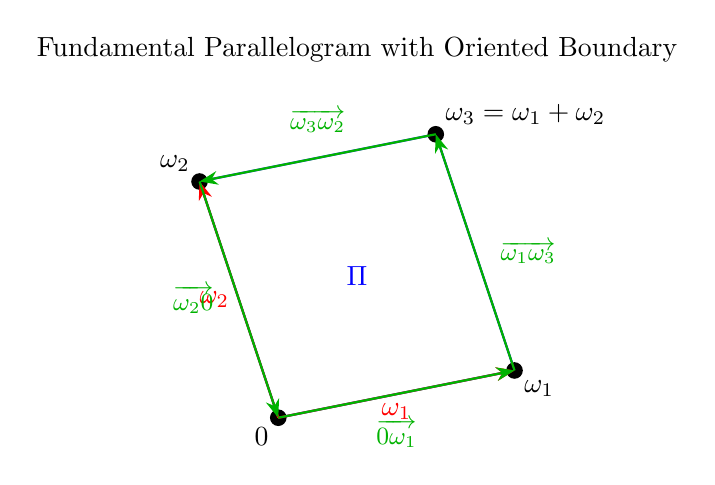
\begin{tikzpicture}[scale=2]
			% Draw the fundamental parallelogram
			\draw[thick, blue] (0,0) -- (1.5,0.3) -- (1,1.8) -- (-0.5,1.5) -- cycle;
			
			% Mark and label the vertices
			\fill[black] (0,0) circle (1.5pt);
			\node[below left] at (0,0) {$0$};
			
			\fill[black] (1.5,0.3) circle (1.5pt);
			\node[below right] at (1.5,0.3) {$\omega_1$};
			
			\fill[black] (-0.5,1.5) circle (1.5pt);
			\node[above left] at (-0.5,1.5) {$\omega_2$};
			
			\fill[black] (1,1.8) circle (1.5pt);
			\node[above right] at (1,1.8) {$\omega_3 = \omega_1 + \omega_2$};
			
			% Draw and label the lattice vectors
			\draw[-{Stealth}, thick, red] (0,0) -- (1.5,0.3);
			\node[below, red] at (0.75,0.15) {$\omega_1$};
			
			\draw[-{Stealth}, thick, red] (0,0) -- (-0.5,1.5);
			\node[left, red] at (-0.25,0.75) {$\omega_2$};
			
			% Draw directed edges with arrows to show orientation
			\draw[-{Stealth}, thick, green!70!black] (0,0) -- (1.5,0.3);
			\draw[-{Stealth}, thick, green!70!black] (1.5,0.3) -- (1,1.8);
			\draw[-{Stealth}, thick, green!70!black] (1,1.8) -- (-0.5,1.5);
			\draw[-{Stealth}, thick, green!70!black] (-0.5,1.5) -- (0,0);
			
			% Label the boundary segments
			\node[below, green!70!black, font=\small] at (0.75,0.05) {$\overrightarrow{0\omega_1}$};
			\node[right, green!70!black, font=\small] at (1.35,1.05) {$\overrightarrow{\omega_1\omega_3}$};
			\node[above, green!70!black, font=\small] at (0.25,1.75) {$\overrightarrow{\omega_3\omega_2}$};
			\node[left, green!70!black, font=\small] at (-0.35,0.75) {$\overrightarrow{\omega_2 0}$};
			
			% Add fundamental domain label
			\node[blue] at (0.5,0.9) {$\Pi$};
			
			% Add title
			\node[above] at (0.5,2.2) {Fundamental Parallelogram with Oriented Boundary};
		\end{tikzpicture}
	\end{center}
	
	To prove (a), it remains to show that $\int_{\partial\Pi} f(\xi) d\xi = 0$.
	
	Note that
	\begin{align}
		\int_{\partial\Pi} f(\xi) d\xi &= \int_{\overrightarrow{0\omega_1}} f(\xi) d\xi + \int_{\overrightarrow{\omega_1, \omega_1+\omega_2}} f(\xi) d\xi \\
		&\quad + \int_{\overrightarrow{\omega_1+\omega_2, \omega_2}} f(\xi) d\xi + \int_{\overrightarrow{\omega_2, 0}} f(\xi) d\xi \\
		&= \underbrace{\left(\int_{\overrightarrow{0\omega_1}} - \int_{\overrightarrow{\omega_2, \omega_1+\omega_2}}\right)}_{\mathrm{I}} + \underbrace{\left(\int_{\overrightarrow{\omega_1, \omega_1+\omega_2}} - \int_{\overrightarrow{0\omega_2}}\right)}_{\mathrm{II}}
	\end{align}
	
	We will show that $\mathrm{I} = 0$ and $\mathrm{II} = 0$ follows easily.
	
	For $\mathrm{I}$, parametrize $\overrightarrow{0\omega_1}$ by $\xi(t) = t\omega_1$, where $\xi: [0,1] \xrightarrow{\cong} \overrightarrow{0\omega_1}$. Then we have
	\begin{align}
		\int_{\overrightarrow{0\omega_1}} f(\xi) d\xi &\overset{\text{def}}{=} \int_0^1 f(t\omega_1) \omega_1 dt \\
		&= \int_0^1 f(t\omega_1 + \omega_2) \omega_1 dt \quad \text{(by ellipticity)} \\
		&= \int_{\overrightarrow{\omega_2, \omega_1+\omega_2}} f(\xi) d\xi
	\end{align}
	
	\textbf{Part (b):} Consider $g(z) = \frac{f'(z)}{f(z)}$, which is elliptic. Apply part (a): $\text{Res}\left(\frac{f'}{f}\right) = \text{ord}_a(f)$, so
	\[
	\sum_{a \in \Pi} \text{ord}_a(f) = \sum_{a_i \in \Pi} \text{Res}(g, a_i) = 0
	\]
	
\textbf{Part (c):} The proof is equivalent to showing $\sum'_{a \in \Pi} \text{ord}_a(f) \cdot a \equiv 0 \pmod{L}$.

Proof by Residue Theorem applied to $z\frac{f'(z)}{f(z)}$. First, we analyze the poles of $\frac{f'(z)}{f(z)}$:


 If $a$ is a zero of $f$ of order $m > 0$, then near $a$ we have $f(z) = (z-a)^m g(z)$ where $g(a) \neq 0$. Thus 
	\[
	\frac{f'(z)}{f(z)} = \frac{m(z-a)^{m-1}g(z) + (z-a)^m g'(z)}{(z-a)^m g(z)} = \frac{m}{z-a} + \frac{g'(z)}{g(z)}
	\]
	Since $g$ is holomorphic and nonzero at $a$, we see that $\frac{f'}{f}$ has a simple pole at $a$ with residue $m = \text{ord}_a(f)$.
	
 If $b$ is a pole of $f$ of order $n > 0$, then near $b$ we have $f(z) = (z-b)^{-n} h(z)$ where $h(b) \neq 0$. Thus
	\[
	\frac{f'(z)}{f(z)} = \frac{-n(z-b)^{-n-1}h(z) + (z-b)^{-n} h'(z)}{(z-b)^{-n} h(z)} = \frac{-n}{z-b} + \frac{h'(z)}{h(z)}
	\]
	So $\frac{f'}{f}$ has a simple pole at $b$ with residue $-n = \text{ord}_b(f)$.


Therefore, $\frac{f'(z)}{f(z)}$ has only simple poles, and at each point $a \in \Pi$ (zero or pole of $f$), the residue is exactly $\text{ord}_a(f)$.

Now, using the formula $\text{Res}(gh; a) = g(a)\text{Res}(h; a)$ where $h$ has a simple pole at $a$ and $g$ is holomorphic at $a$, we get:

\[
\frac{1}{2\pi i} \int_{\partial\Pi} \xi \frac{f'(\xi)}{f(\xi)} d\xi = \sum'_{a \in \Pi} \text{Res}\left(z\frac{f'(z)}{f(z)}, a\right) = \sum'_{a \in \Pi} a \cdot \text{ord}_a(f)
\]

We have
\[
\int_{\partial\Pi} \xi \frac{f'(\xi)}{f(\xi)} d\xi = \underbrace{\int_{\overrightarrow{0\omega_1}} - \int_{\overrightarrow{\omega_2, \omega_1+\omega_2}}}_{\mathrm{I}'} + \underbrace{\int_{\overrightarrow{\omega_1, \omega_1+\omega_2}} - \int_{\overrightarrow{0\omega_2}}}_{\mathrm{II}'}
\]

Using the parametrization in part (a):
\begin{align}
	\int_{\overrightarrow{0\omega_1}} \xi \frac{f'}{f} d\xi &= \int_0^1 (t\omega_1) \frac{f'(t\omega_1)}{f(t\omega_1)} \omega_1 dt \\
	\int_{\overrightarrow{\omega_2, \omega_1+\omega_2}} \xi \frac{f'}{f} d\xi &= \int_0^1 (t\omega_1 + \omega_2) \frac{f'(t\omega_1 + \omega_2)}{f(t\omega_1 + \omega_2)} \omega_1 dt
\end{align}

Then
\begin{align}
	\mathrm{I}' 
	&= -\omega_2 \int_{0}^{1} \frac{f'(t\omega_1)}{f(t\omega_1)}\,\omega_1\, dt
	\tag{18}\\[4pt]
	&= -\omega_2 \int_{\overrightarrow{0\omega_1}} 
	\frac{f'(\xi)}{f(\xi)}\, d\xi
	\tag{19}\\[4pt]
	&= -\omega_2 \int_{\overrightarrow{0\omega_1}}
	d(\log f(\xi))
	\tag{20}\\[4pt]
	&= -\omega_2 
	\bigl[\log f(\omega_1)-\log f(0)\bigr]
	\tag{21}\\[4pt]
	&= -\omega_2 (2\pi i n),
	\qquad n\in\mathbb{Z},
	\tag{22}
\end{align}

\noindent
since \( f(\omega_1) = f(0) \Rightarrow 
e^{\log f(\omega_1)-\log f(0)} = 1 = e^{2\pi i n} \).
where $\log f$ can be defined near $0$ and analytically continued along a neighborhood of $\overrightarrow{0\omega_1}$.

Thus $\frac{1}{2\pi i}\mathrm{I}' = -n\omega_2$. Similarly, we can show that
\[
\frac{1}{2\pi i} \int_{\partial\Pi} \xi \frac{f'(\xi)}{f(\xi)} d\xi = n_1\omega_1 + n_2\omega_2, \quad \exists n_1, n_2 \in \Z
\]
so it falls in $L$.
\end{proof}
	
	
	
	
	
	
	
	
	
	
	
	
	
	
	
	
	
	
	
	
	
\end{document}